\subsection{Apparatus}
\label{sec:test:apparatus}

\begin{figure}
  \centering
  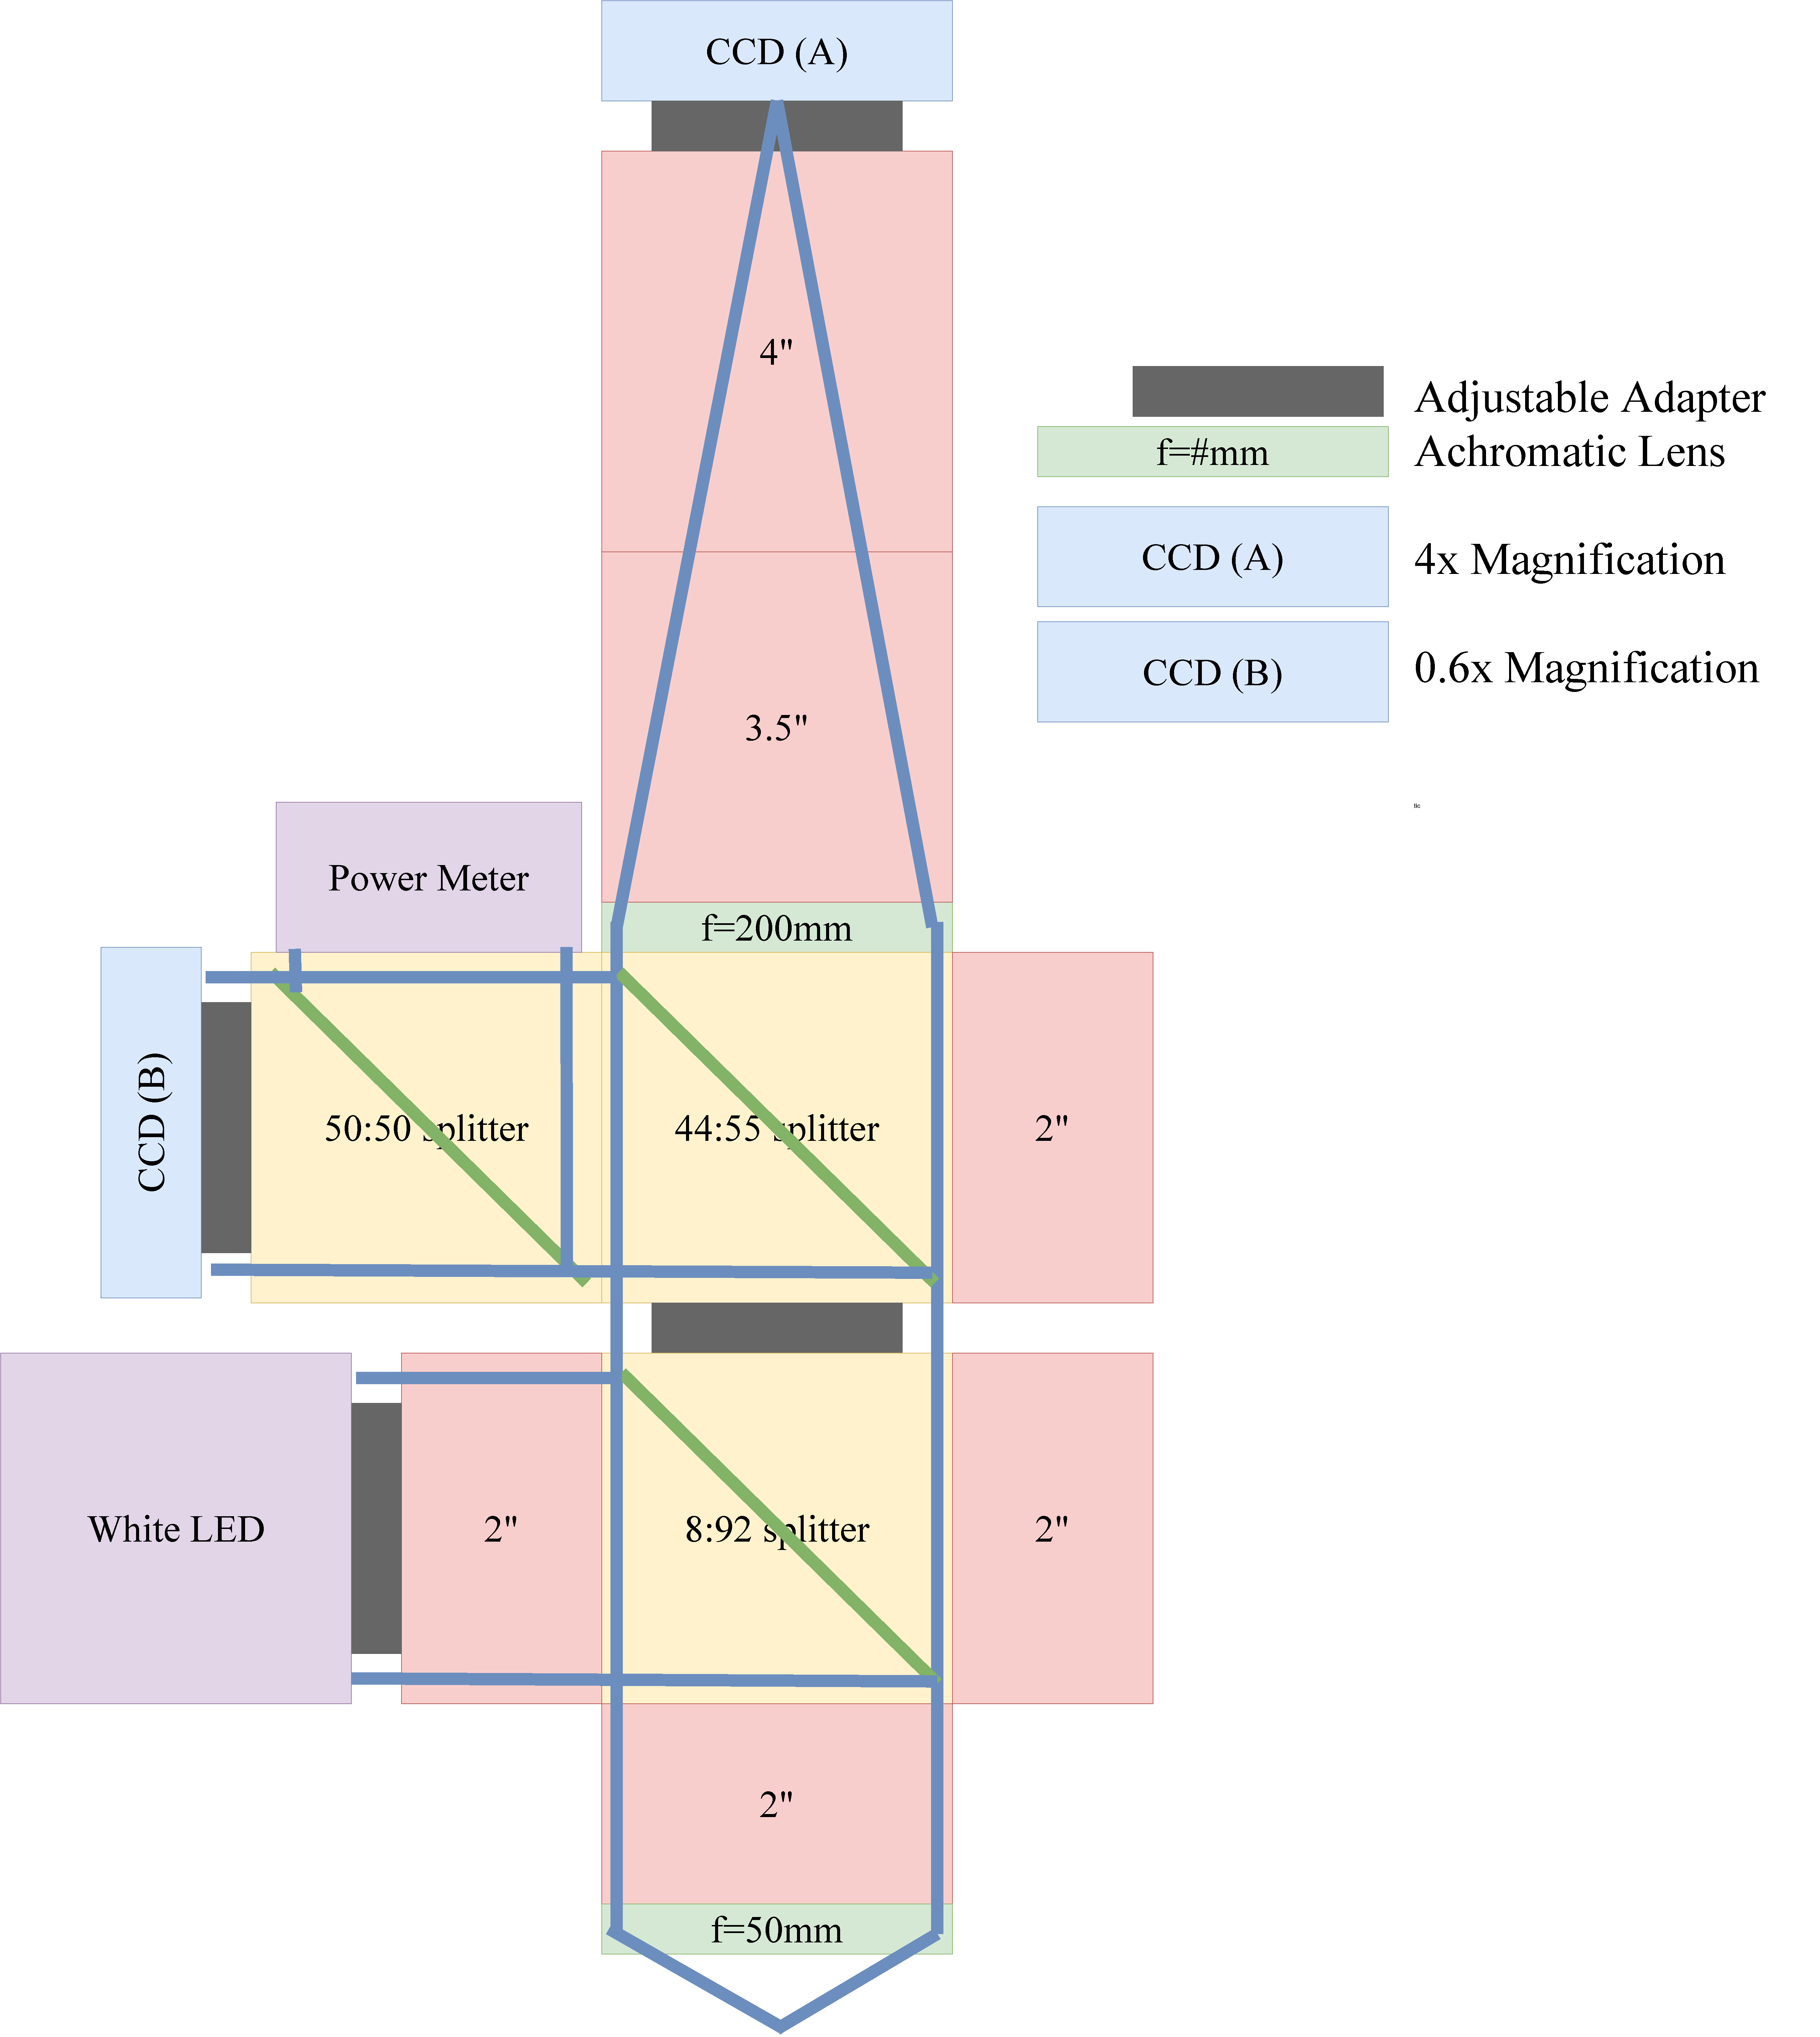
\includegraphics[width=0.6\textwidth]{Figures/angus_bruce/apparatus_microandnano1.pdf}
  \caption{Schematic of the Test Apparatus. The device to be tested is placed at the focal point below the lens with a focal length of $50mm$}
  \label{fig:apparatus}
\end{figure}

Figure \ref{fig:apparatus} shows a schematic of the apparatus used to test the LED. The measured power on the power meter will not be absolute but rather as an indication relative to other measurements on the same apparatus. This is true for two reasons. The light goes through beam splitters before being measured. Also, the light from the LED emits light in all directions so only a fraction of the light pass through the apparatus in the first place.
